\documentclass{scrartcl}

\usepackage{amssymb}
\usepackage{amsmath}
\usepackage{tikz}
\usetikzlibrary{calc,intersections,through,backgrounds,patterns}
\usetikzlibrary{decorations.text, decorations.markings, fit, arrows, arrows.meta}

\begin{document}

	\begin{figure}
	%	\centering
	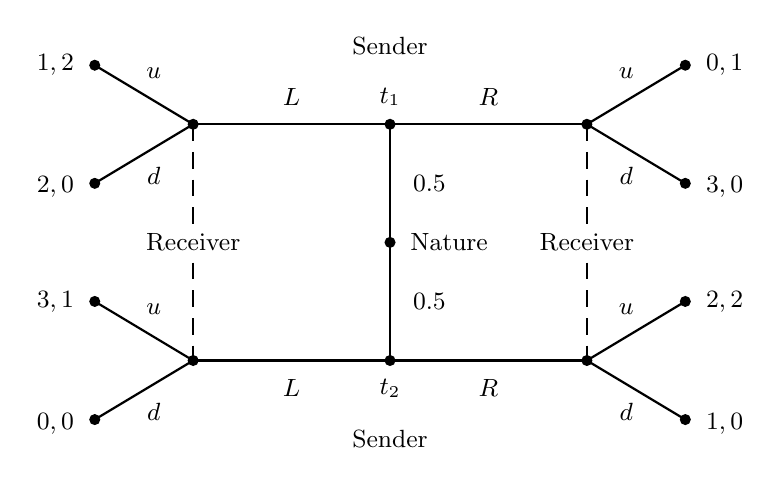
\begin{tikzpicture}
	\fill (-3.75,2.25) circle (2pt);	%upper left node, top
	\fill (-3.75,0.75) circle (2pt);	%upper left node, bottom
		\draw[thick] (-2.5,1.5)--(-3.75,2.25);
		\draw[thick] (-2.5,1.5)--(-3.75,0.75);
	\fill (-3.75,-2.25) circle (2pt);	%lower left node, top
	\fill (-3.75,-0.75) circle (2pt);	%lower left node, bottom
		\draw[thick] (-2.5,-1.5)--(-3.75,-2.25);
		\draw[thick] (-2.5,-1.5)--(-3.75,-0.75);
	
	\fill (-2.5,1.5) circle (2pt);	%top horizontal line, left
	\fill (2.5,1.5) circle (2pt);	%top horizontal line, right
	
	\fill (0,1.5) circle (2pt);		%top center
	\fill (0,0) circle (2pt);		%center
	\fill (0,-1.5) circle (2pt);	%bottom center
	
	\fill (-2.5,-1.5) circle (2pt);	%bottom horizontal line, left
	\fill (2.5,-1.5) circle (2pt);	%bottom horizontal line, right
	
	\fill (3.75,2.25) circle (2pt);		%upper right node, top
	\fill (3.75,0.75) circle (2pt);		%upper right node, bottom
		\draw[thick] (2.5,1.5)--(3.75,2.25);
		\draw[thick] (2.5,1.5)--(3.75,0.75);
	\fill (3.75,-2.25) circle (2pt);	%lower right node, top
	\fill (3.75,-0.75) circle (2pt);	%lower right node, bottom
		\draw[thick] (2.5,-1.5)--(3.75,-2.25);
		\draw[thick] (2.5,-1.5)--(3.75,-0.75);
	
	\node at (0,2.5)      {{\small Sender}};		%can remove if preferred
	\node at (-1.25,1.85) {{\small $L$}};
	\node at (1.25,1.85)  {{\small $R$}};
	\node at (0,1.85)     {{\small $t_1$}};
	\node at (0.5,0.75)   {{\small 0.5}};
	\node at (0.75,0) 	  {{\small Nature}};
	\node at (0.5,-.75)   {{\small 0.5}};
	\node at (0,-1.85)    {{\small $t_2$}};
	\node at (-1.25,-1.85){{\small $L$}};
	\node at (1.25,-1.85) {{\small $R$}};
	\node at (0,-2.5)     {{\small Sender}};		%can remove if preferred
	
	\draw[thick] (0,1.5)--(0,-1.5);			%vertical center
	\draw[thick] (-2.5,1.5)--(2.5,1.5);		%top
	\draw[thick] (-2.5,-1.5)--(2.5,-1.5);	%bottom
	%
	\draw[thick,dash pattern=on 6pt off 4pt] (-2.5,1.5)--(-2.5,-1.5);
	\draw[thick,dash pattern=on 6pt off 4pt]  (2.5,1.5)--(2.5,-1.5);
		\node[fill=white] at (-2.5,0) {{\small Receiver}};
		\node[fill=white] at  (2.5,0) {{\small Receiver}};
	
	%optional - probabilities
%	\node at (-2.3,1.75)   {{\scriptsize [$p$]}};
%	\node at  (2.3,1.75)   {{\scriptsize [$q$]}};
%	\node at (-2.15,-1.75) {{\scriptsize [$1\!-\!p$]}};
%	\node at  (2.15,-1.75) {{\scriptsize [$1\!-\!q$]}};
	
	%D's \& U's
	\node at (-3, 2.15) {{\small $u$}};
	\node at (-3, 0.85) {{\small $d$}};
	\node at (-3,-0.85) {{\small $u$}};
	\node at (-3,-2.15) {{\small $d$}};
	%
	\node at (3, 2.15) {{\small $u$}};
	\node at (3, 0.85) {{\small $d$}};
	\node at (3,-0.85) {{\small $u$}};
	\node at (3,-2.15) {{\small $d$}};
	
	%payoffs
	\node at (-4.25, 2.25) {{\small $1,2$}};
	\node at (-4.25, 0.70) {{\small $2,0$}};
	\node at (-4.25,-2.30) {{\small $0,0$}};
	\node at (-4.25,-0.75) {{\small $3,1$}};
	%
	\node at (4.25, 2.25) {{\small $0,1$}};
	\node at (4.25, 0.70) {{\small $3,0$}};
	\node at (4.25,-2.30) {{\small $1,0$}};
	\node at (4.25,-0.75) {{\small $2,2$}};
	
	%alternative payoffs
%	\node at (-4.25, 2.25) {{\small $1,3$}};
%	\node at (-4.25, 0.70) {{\small $4,0$}};
%	\node at (-4.25,-2.30) {{\small $2,4$}};
%	\node at (-4.25,-0.75) {{\small $0,1$}};
	%
%	\node at (4.25, 2.25) {{\small $2,1$}};
%	\node at (4.25, 0.70) {{\small $0,0$}};
%	\node at (4.25,-2.30) {{\small $1,0$}};
%	\node at (4.25,-0.75) {{\small $1,2$}};
	
	%alternative - centered "Nature"
%	\fill[white] (-0.001,0.755) circle (0.8pt);
%	\fill[white] (-0.001,-0.945) circle (0.8pt);
%	\node at (0,0.85)   {{\small 0.5}};
%	\node at (0,-.85)   {{\small 0.5}};
%	\draw[line width=7pt, color=white] (-0.3,-0.37)--(0.3,-0.37);		%manual fill behnd "Nature"
%	\node at (0,-0.35) 	  {{\small Nature}};	
	\end{tikzpicture}
	%	\caption{...}
	\end{figure}

\end{document}